% 1. Introduction
% ---------------
% 1) Protocoles en couches
% 2) Modèle OSI
% 3) Couches OSI
% 4) Fonctionnement du modèle OSI
% 5) IEEE802.15.4
% 6) Stratégies d'implémentation
\section{Modèle OSI et concepts liés}
\begin{itemize}
    \item ISO: International Organization for Standardization ($\xrightarrow{\text{create}}$ OSI)
    \item OSI: Open Systems Interconnection
    \item SDU: Service Data Unit
    \item PDU: Protocol Data Unit
\end{itemize}
« Le modèle OSI ne spécifie pas un protocole. Il s'agit plutôt d'un framework pour la spécification de protocole. »

OSI introduit la notion de \textbf{service} (\textbf{SAP} - Service Access Point) avec un \textcolor{Periwinkle}{Service User} et un \textcolor{BurntOrange}{Service Provider}.
\begin{figure}[H]
    \centering
    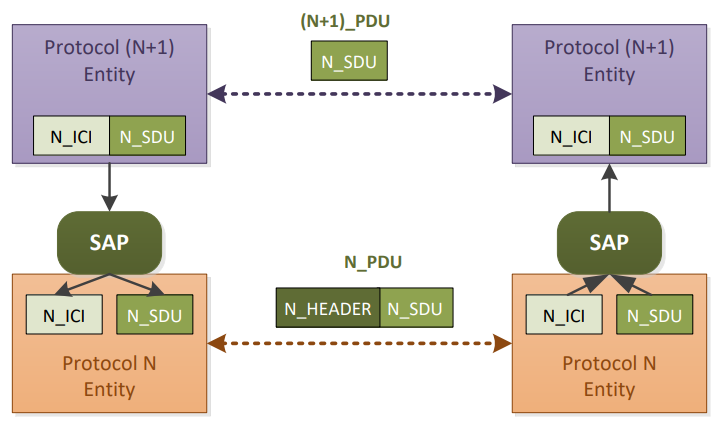
\includegraphics[width=.8\linewidth]{figures/OSI_SAP.png}
\end{figure}

Basé sur \textbf{4 primitives} de service.
\begin{figure}[H]
    \centering
    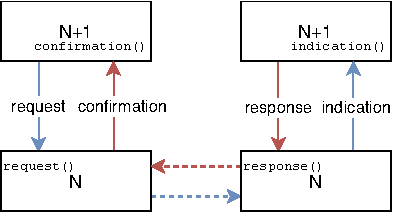
\includegraphics[width=5cm]{figures/4primitives.pdf}
\end{figure}

Modèle OSI complet :
\begin{figure}[H]
    \centering
    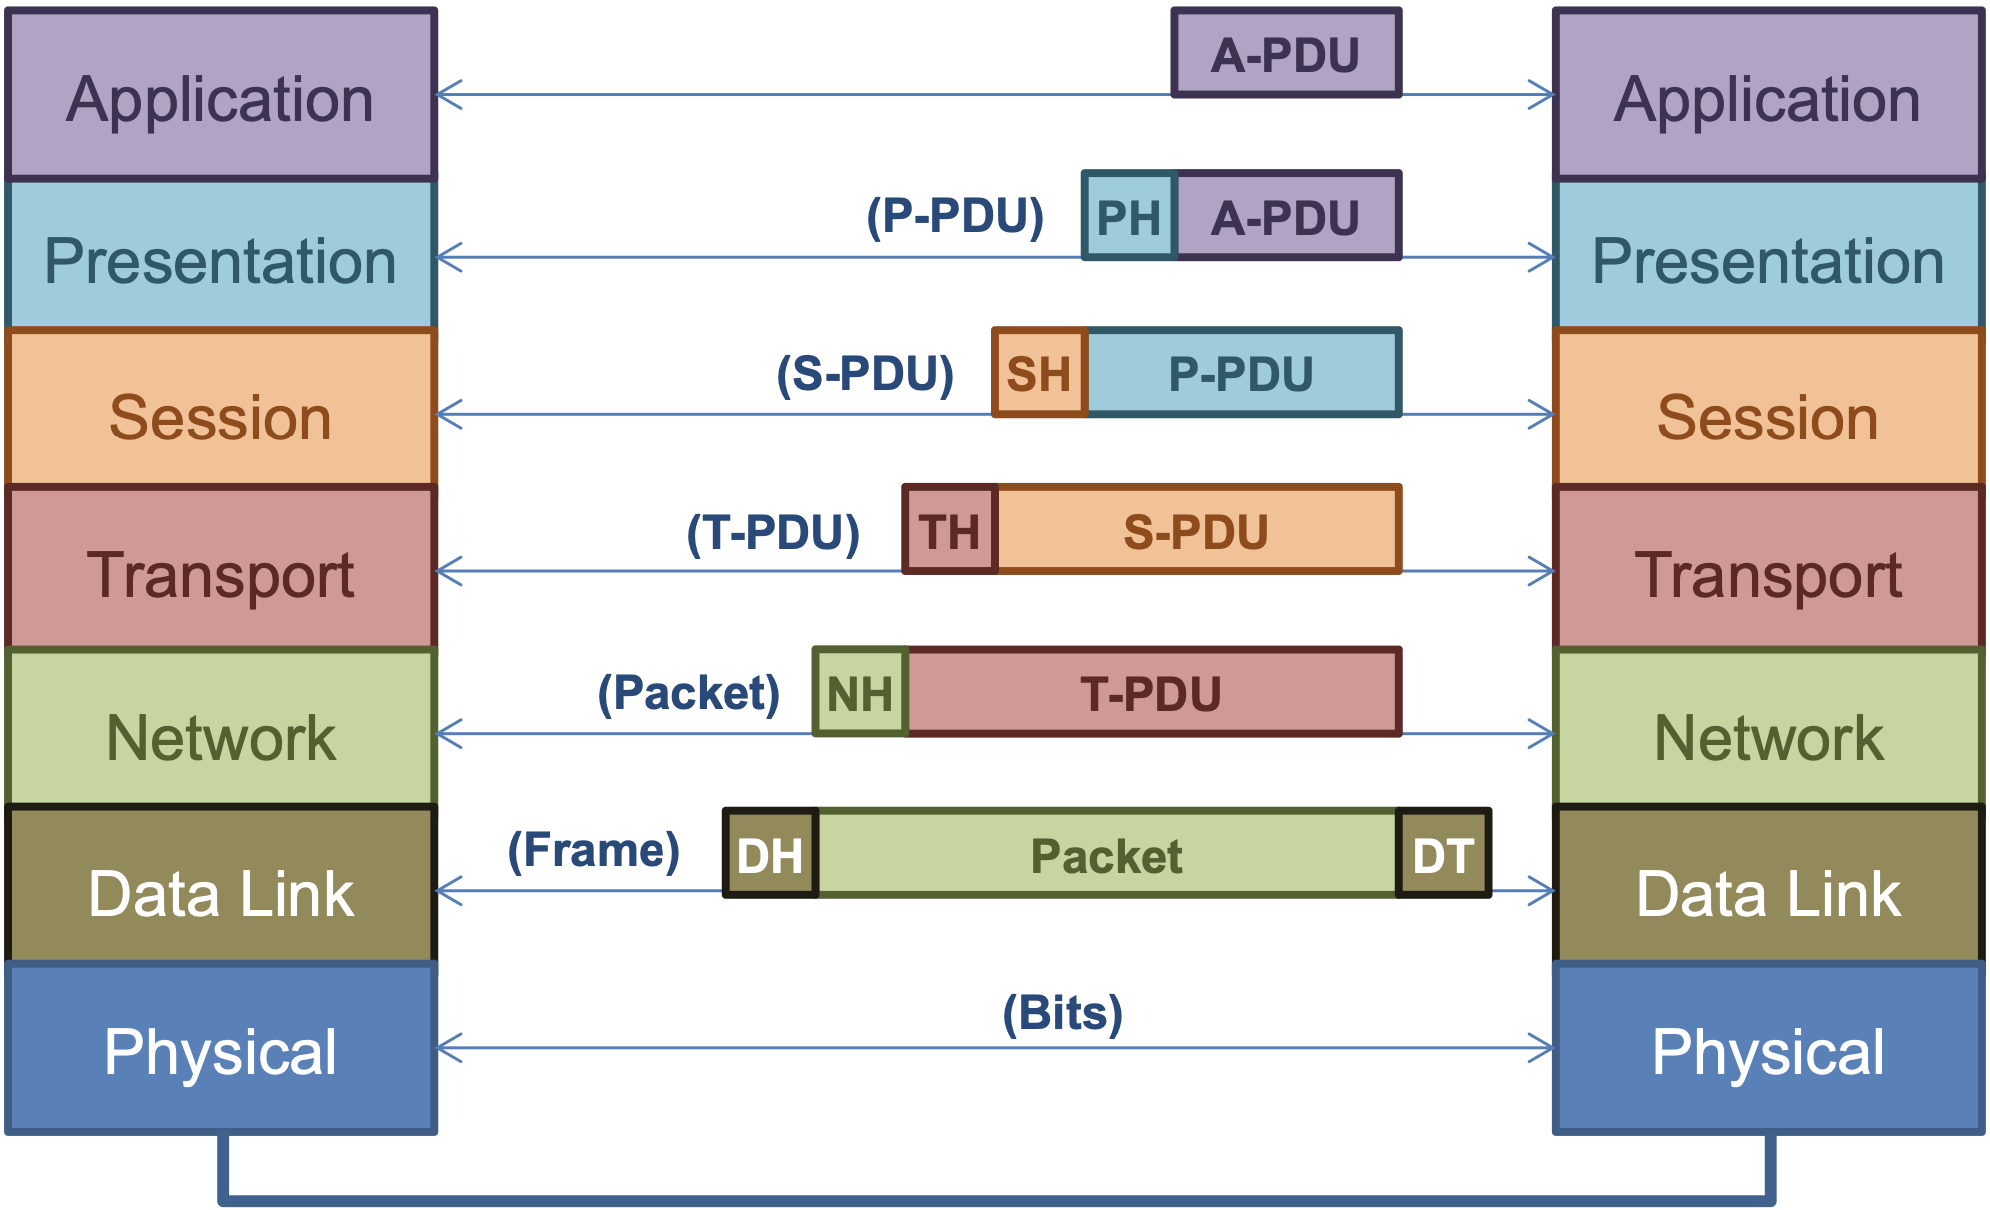
\includegraphics[width=.7\linewidth]{figures/OSI_model_operation.png}
\end{figure}
